\documentclass[11pt,a4paper]{article}
\usepackage[margin=23mm,headheight=15pt]{geometry}
\usepackage{fontspec}
\setmainfont{Times New Roman}
\setsansfont{Arial}
\usepackage{amsmath,amssymb,graphicx,booktabs,array,tabularx,longtable,caption,xcolor,fancyhdr,enumitem,placeins}
\usepackage[numbers,sort&compress]{natbib}
\usepackage[colorlinks=true,linkcolor=teal!55!black,citecolor=teal!55!black,urlcolor=teal!55!black]{hyperref}
\definecolor{navy}{HTML}{193447}
\definecolor{pale}{HTML}{EDF4F5}
\usepackage{titlesec}
\titleformat{\section}{\large\sffamily\bfseries\color{navy}}{}{0em}{}
\setlength{\parindent}{0pt}
\setlength{\parskip}{6pt}
\raggedbottom
\setlength{\emergencystretch}{3em}
\widowpenalty=10000\clubpenalty=10000
\renewcommand{\topfraction}{.95}\renewcommand{\bottomfraction}{.85}\renewcommand{\textfraction}{.05}\renewcommand{\floatpagefraction}{.75}
\renewcommand{\arraystretch}{1.16}
\captionsetup{font=small,labelfont=bf,justification=raggedright,singlelinecheck=false}
\pagestyle{fancy}\fancyhf{}\fancyhead[L]{\small\sffamily EVIDENCE TO EXPERIMENT}\fancyhead[R]{\small\sffamily 18 November 2026}\fancyfoot[C]{\thepage}
\renewcommand{\headrulewidth}{0.3pt}
\graphicspath{{figures/}}
\newcounter{boxnum}
\newcommand{\boxlabel}{Box}
\usepackage[mathlines]{lineno}
\setlength{\linenumbersep}{8pt}
\renewcommand\linenumberfont{\normalfont\tiny\sffamily}
\begin{document}\runninglinenumbers
{\small\sffamily\color{navy} PERSPECTIVE | EVIDENCE SYNTHESIS}\par\medskip
{\LARGE\bfseries\raggedright Shared and separable motor learning: reconciling transfer, dissociation and error attribution\par}\bigskip
{\normalsize JiaHao Wu and Long Zeng\par}
{\small Tsinghua Shenzhen International Graduate School, Tsinghua University, Shenzhen, China\par}\medskip
\hypersetup{pdfauthor={JiaHao Wu; Long Zeng}}
{\small Correspondence: Long Zeng, \href{mailto:zenglong@sz.tsinghua.edu.cn}{zenglong@sz.tsinghua.edu.cn}\par}\medskip
\section{Abstract}
Motor learning transfers between planned actions and corrective responses, yet also separates across sensory channels and contexts. We argue that these findings describe coupling at different stages of learning. Integrating evidence across sensory inputs, control outputs and timescales explains how separable memories can support shared behaviour. Two worked cases show how temporal mixing and perceptual reporting change the measurements needed to distinguish explanations. Public-data reanalyses support richer temporal responses while exposing unstable architecture rankings. An experiment-level evidence map translates this synthesis into competing predictions, essential controls and targeted measurements for motor neuroscience and embodied control.

\section{The problem revealed by a force field}
Learning a sideways force field changes both the forces prepared before a reach and the corrections made during it. Other experiments selectively alter one response or reveal memories specific to vision and proprioception. Together, these findings ask how learning can be shared across actions while remaining separable across inputs and conditions. Force-field adaptation makes this question concrete: channel trials measure anticipatory compensation, perturbations reveal feedback responses, and muscle activity constrains the contribution of body mechanics. \cite{wagner2008,maeda2018,yousif2012,hayashi2020}

We argue that sharing is a relation that must be specified across sensory inputs, control outputs and timescales. Distinct sensory learning processes can contribute to both planned and corrective actions. Their relative contributions depend on error attribution, retention and the context in which a memory is expressed. This organization explains why transfer and dissociation can coexist: the same learning system can couple outputs under one comparison and separate them under another.

The practical consequence is a change in what experiments compare. A transfer result motivates a crossed training--test-context comparison; a changing output ratio motivates paired temporal responses; a localization shift motivates independent calibration of what the report measures. We develop these consequences through the force-field case, connect them to a 29-entry evidence map, and use worked constructions and public-data reanalyses to establish which distinctions each measurement can resolve. The resulting contribution is an explicit route from an apparent contradiction to a competing prediction and an experimental choice.


\begin{figure}[!htbp]\centering
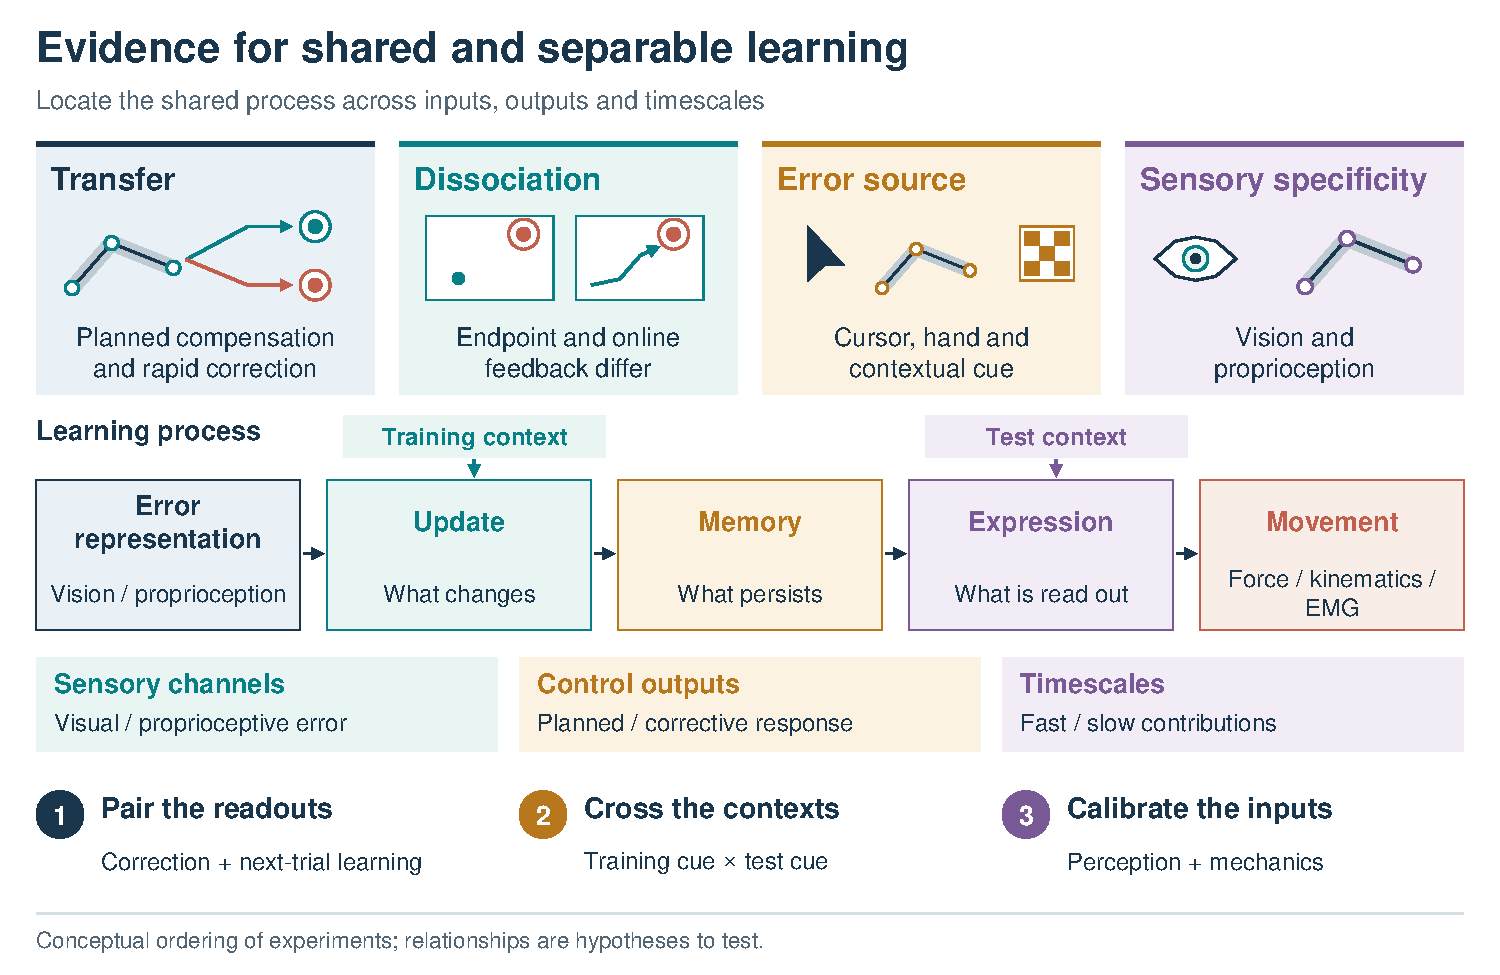
\includegraphics[width=\textwidth]{figure1_en.pdf}
\caption{Evidence streams and proposed integration. The four observations constrain different stages of learning and three independent dimensions: sensory channels, control outputs and timescales. The pathway organizes experimental comparisons. Native PowerPoint text, shapes and connectors depict conceptual relationships to be tested.}
\end{figure}
\section{How the evidence map was constructed}
The map is a purposive critical synthesis of experiments that connect at least two relevant measurements, selectively manipulate a learning condition, or expose an alternative implementation. The updated map additionally searches for target-error, uncertainty, attention and perceptual-error findings that challenge its central claims. Eight claim cards record support, counterevidence to the stated or stronger proposition, scope and the resulting experimental choice. This adversarial audit is documented in the atlas and search log. Its core is human upper-limb adaptation; computational source-inference and recurrent-network studies establish explicit competitors. Entries record the manipulation, measurement, observed result, supported inference, residual account and proposed discriminating test. A source locator identifies the experiment, figure or results section supporting each entry. Original findings and our proposed tests occupy separate fields. The search and source check were updated through 17 November 2026; the 2026 eLife item is labelled as reviewed preprint version 1. \cite{makino2026}

The unit of synthesis is an experimental contrast with a defined readout. Results measured as a 50--100 ms muscle response, a 251--350 ms visually evoked force, or a next-trial aftereffect retain their original timing and meaning. We use study-specific controls to judge each inference. For example, Cluff and Scott controlled background activation through a probe target, making their evidence more informative than a correlation between two unconstrained outputs. The atlas preserves such design strengths alongside the remaining alternatives. It provides an auditable argument rather than a pooled effect estimate; heterogeneous outcomes are compared by their causal role in the experiment. \cite{cluff2013,maeda2018,kasuga2015}

\section{Transfer establishes cross-output access to learned dynamics}
Wagner and Smith showed that corrective responses incorporated learned force-field dynamics (E01). Maeda and colleagues provided a complementary manipulation of the arm itself: shoulder fixation reduced the shoulder commands required for voluntary elbow movements, and this learning transferred to long-latency responses measured with the shoulder free (E02). Training perturbation responses subsequently transferred in the reverse direction to voluntary reaching (E03). Cluff and Scott measured load-specific changes in long-latency responses while controlling muscle activation at a probe target (E08). These experiments support a robust common statement: experience acquired in one control setting changes how another setting responds to limb dynamics. \cite{wagner2008,maeda2018,maeda2020,cluff2013}

This common statement constrains candidate mechanisms. A shared dynamics estimate supplies both outputs with updated predictions. Distinct adaptive pathways can communicate an update or receive a common teaching signal. A recurrent controller can embed dynamics-sensitive responses in its policy. A feedback-trained recurrent implementation has reproduced several behavioural and neural learning features, providing a concrete alternative to explicit predictor architectures (E21). The critical comparison is therefore the joint prediction across outputs and interventions after their normal behaviour is matched. \cite{feulner2025}

Transfer also depends on the test. A cue can select a stored memory or change its gain at readout. The COIN framework and its evoked-recovery experiments demonstrate how contextual inference affects memory expression and updating (E19). A two-by-two crossing of training cue and test cue directly exposes this ambiguity: a test-cue effect on the first error-free probe identifies an expression contribution; a training-cue effect that survives a common test cue motivates comparison of acquisition, retention and persistent input recalibration. Such a design assigns different observations to different stages of the transfer process. \cite{coin2021}

\section{Dissociation identifies the conditions of coupling}
Yousif and Diedrichsen manipulated temporal consistency while matching the counts of exposure-trial types. Consistent experience altered structural learning in both feedforward and feedback measurements; inconsistent experience altered feedback structure without the corresponding feedforward structural change (E04). This result makes disturbance history part of the mechanism. A model with a single unconditional update applied identically to both readouts must explain why temporal organization changes the relationship. Distinct timescales, context selection and selective updates offer explicit alternatives. \cite{yousif2012}

Kasuga and colleagues manipulated access to online visual consequences during mirror-reversed reaching (E05). Endpoint feedback supported better feedforward performance, while continuous feedback produced stronger attenuation of inappropriate corrective responses. The measured feedback response was a visually evoked force in a later window than the long-latency mechanical responses above. Mirror reversal also changes the required policy mapping. These differences specify a valuable contrast: knowledge transfer under altered dynamics and acquisition of a new feedback mapping place different demands on experience. Comparing them requires matched exposure, training duration and baseline performance. \cite{kasuga2015}

Timescale adds a further distinction. Crevecoeur and colleagues observed field-specific adjustment during ongoing movements exposed to unanticipated dynamics (E11). Such within-movement adaptation can improve an endpoint before a persistent next-trial change is established. A paired design therefore asks both whether the current correction changes and what survives into a subsequent probe. Delay-resolved tests then distinguish transient control adjustment from slower retention processes. \cite{crevecoeur2020}

\section{Error attribution depends on the candidate cause}
The word ``external'' covers biologically different causes. A display displacement that can be discounted, an external force that will recur, and an unexpected object mass imply different useful responses. Likewise, ``internal'' can refer to random execution noise or a persistent change in limb dynamics. Berniker and Kording formalized the consequences: inferred body and world changes predict different generalization patterns (E13). Wei and Kording related nonlinear error sensitivity to inferred error relevance (E14). These studies motivate recording source, persistence and behavioural relevance separately. \cite{berniker2008,wei2009}

Gastrock and colleagues revealed a visuomotor rotation through cursor jumps or hand visibility (E15). Aftereffects decreased, while the hand-view active-minus-passive localization estimate was near zero and proprioceptive recalibration persisted; the direct control-versus-hand-view report contrast remained uncertain. This identifies component-selective consequences of revealing a display distortion. Hand visibility simultaneously changes available sensory information, so a cue-only manipulation with matched visibility supplies the next useful contrast. \cite{external2020}

Kim and colleagues compared externally imposed rotations with matched internally generated movement errors and found greater adaptation to the externally imposed errors (E16). Here the internal category was movement variability, and the proposed causal-inference model estimated whether an external perturbation had occurred. Together, these findings support a conditional synthesis: learning depends on which latent cause the evidence supports and which behavioural component is measured. The prediction ``external attribution reduces learning'' loses the distinctions needed to explain both experiments. A stronger test crosses source credibility with persistence while matching physical and perceived error, then measures perceptual and motor consequences separately. \cite{piece2025}

\section{Sensory-specific learning can support shared control outputs}
Hayashi and colleagues independently varied visual and proprioceptive errors, including opposing-error conditions (E17). Nonlinear aftereffects and modality-dependent learning dynamics supported their account of distinct sensory memories with interacting error processing. This evidence constrains the input dimension of learning. Both sensory-specific states could still contribute to planned compensation and corrective control. A statement about separate visual and proprioceptive memories and a statement about transfer between feedforward and feedback control can therefore hold within one architecture. \cite{hayashi2020}

Hoffmann and colleagues brought the two dimensions into the same experiment (E18). Scaling visual displacement during force perturbations changed online corrections more consistently than subsequent aftereffects, and instructions to control the hidden hand removed a residual visual influence on adaptation. The task goal affects how sensory evidence relates to correction and learning. A crossed target-by-reliability experiment should therefore calibrate perceived displacement separately and evaluate the untrained combinations with fixed learned parameters. \cite{hoffmann2023}

Izawa and Shadmehr demonstrate why adding a sensory consequence is useful: sensory-error and reward-driven learning produced different sensory remapping (E12). Gastrock and colleagues extend this logic with active and passive localization. These measurements can reveal an input or prediction change that a reach endpoint misses. The subtraction between active and passive reports is itself a measurement model, requiring matched reporting demands and an assessment of localization reliability. \cite{izawa2011,external2020}

\section{What the integration adds}
The synthesis links three established advances. Hayashi et al. showed how sensory-specific memories can combine at output; Smith et al. established interacting adaptation processes with different timescales; Heald et al. explained how contextual inference changes memory updating and expression. Transfer experiments constrain a further axis: learned dynamics influence both anticipatory and corrective control. Each contribution identifies a different relation within learning. Their conjunction yields a specific account of the apparent contradiction: sensory-specific acquisition can coexist with cross-output access, while temporal mixtures and context determine the expression of that access. \cite{hayashi2020,smith2006,coin2021,wagner2008,maeda2020}

The increment is the connection from this joint account to observations that adjudicate among explanations. Consider an early transfer effect followed by a later dissociation. Separate discussion of the studies leaves both shared and separate learning accounts available. The integrated account first asks whether the two studies changed input, test context or measurement delay. At a common input and context, it then asks whether fixed mixtures of fast and slow components reproduce the dissociation. If they do, the decisive comparison becomes a prediction of paired responses at new delays. If the dissociation instead follows the test cue on the first error-free probe, expression becomes the relevant experimental contrast. This progression gives the same observed dissociation different, testable meanings according to the intervention that produced it.

Three changes in experimental inference follow (Table~\ref{tab:synthesis}). An output ratio is replaced by a joint temporal response when multiple timescales are plausible. A perceptual report constrains input-versus-update accounts through measured report loadings. A transfer measurement is interpreted through the separation of training and test contexts. The following sections work through the first two cases and connect all three to experiment-selection rules. The framework's added value is the choice of the next informative comparison, grounded in the controls and observations of the original studies.

\begin{table}[!htbp]\small\caption{From established findings to the experimental increment of this synthesis. The first column credits prior contributions; the next columns state the joint interpretation and the comparison it motivates.}\label{tab:synthesis}
\begin{tabularx}{\textwidth}{>{\raggedright\arraybackslash}X>{\raggedright\arraybackslash}X>{\raggedright\arraybackslash}X}\toprule
\textbf{Established contribution} & \textbf{Joint interpretation} & \textbf{Experimental consequence}\\\midrule
Sensory-specific memories combine at output (Hayashi et al.). & Separate acquisition can support transfer into several control outputs. & Cross sensory error channels with anticipatory and corrective readouts.\\[6pt]
Adaptation contains interacting timescales (Smith et al.). & Fixed mixed readout can generate delay-dependent dissociation. & Predict both outputs at reserved delays; compare common and output-specific dynamics.\\[6pt]
Context affects updating and expression (Heald et al.). & Transfer depends on both the training condition and the condition of measurement. & Cross training and test cues; use the first error-free probe at matched delay.\\[6pt]
Active and passive localization sample different information (Gastrock et al.). & A report constrains input versus updating through its component loadings. & Calibrate report loadings independently and predict joint report-and-motor outcomes.\\[6pt]
\bottomrule\end{tabularx}\end{table}
\section{Temporal mixtures resolve the apparent contradiction}
Distinct sensory memories can contribute to both anticipatory compensation and feedback correction. Each contribution can contain fast and slow components. Consequently, a component that dominates early transfer may decay before a later probe, changing the relationship between outputs while every readout weight remains fixed. This is a concrete mechanism by which transfer and dissociation arise within one architecture. \cite{hayashi2020,smith2006}

In a two-mode worked example, both sensory inputs excite both modes, and the outputs read fixed mixtures. One input's output ratio changes from 1.091 immediately after learning to 1.371 after four error-free retention steps; the other changes from 0.536 to 0.713. The complete matrices and calculation appear in Supplementary Methods SM1. The changing ratio identifies a departure from an effectively one-dimensional response. A fixed mixture of multiple temporal components remains compatible with the observation.

The next experiment therefore measures both outputs at several independent delays and predicts reserved delays or perturbation histories. A model with common temporal modes requires the same decay factors to explain both outputs, with different amplitudes allowed; output-specific modes permit different decay factors. Their predictions should be evaluated at matched sensory exposure, context and mechanics, using independent first probes to measure retention before probe-induced learning. The common recurrence and its measurement requirements are given in SM1. \cite{unlearning2016}

This comparison assigns a precise meaning to temporal coupling. A successful common-mode prediction establishes a common description of measured dynamics. Independently targeted pathway interventions are required to localize the states implementing those dynamics, because shared states and synchronized output-specific copies can reproduce the same response. The experimental decision follows the intended claim: temporal measurements constrain response dynamics; selective interventions constrain neural implementation.

\section{A joint explanation with explicit observables}
The integrated account connects a controlled error to its later consequences in planned and corrective actions. For small perturbations around a specified baseline, write
\begin{equation}\Delta\mathbf y_{t+k}=H(q_{\mathrm{test}})A^kU(q_{\mathrm{train}})E(s)\mathbf e_t+\boldsymbol\epsilon.\label{eq:factor}\end{equation}
The physical error $\mathbf e_t$ enters a sensory representation $E$, updates adaptive states through $U$, persists through $A$, and reaches the measured outputs through $H$. Sensory condition $s$, training context $q_{\mathrm{train}}$ and test context $q_{\mathrm{test}}$ can act at different stages. A visual-specific state and a proprioceptive-specific state may therefore learn differently while both contribute to compensation and correction. This local representation organizes the experimental contrasts; larger perturbations can require nonlinear input, state and output mappings.

The four competing explanations now have explicit locations. A source-dependent scalar gate changes the overall update amplitude. An input account changes the represented error in $E$. A routing account changes the pattern of updating in $U$. An expression account changes the contribution of retained states through $H$. Retention in $A$ determines how each consequence changes with delay. At a single condition, the experiment measures their product. Independently calibrated inputs, crossed contexts and paired time courses test whether the same factorization predicts new conditions.

This formulation organizes the strongest supported conclusion: sensory selectivity and cross-output access can coexist, with context and timescale determining their measured relationship. The joint tests locate changes in that relationship. Selective neural interventions can then ask which physical pathways implement the effective factors. In this way, the integrated account connects behavioural evidence to progressively more specific mechanistic claims.

\section{The counterevidence changes the experiment}
Some disagreements survive the integration and determine additional controls. Tsay et al. found that task error modulated implicit recalibration in the presence of sensory prediction error, with target flicker also attenuating learning (E22). Oza et al. attributed task-error benefits to instruction-sensitive action selection and found dissociable implicit recalibration (E23). Their contrast exposes a concrete dispute over automatic interaction, with target events, instructions and attention differing between protocols. A matched comparison must hold the cursor-error schedule fixed, cross task error with a target-flicker control, and measure aim plus the immediate instructed no-feedback aftereffect. The interaction account predicts a task-error effect in the residual implicit component; strategic addition predicts instruction-sensitive total improvement with a stable implicit component. Aim reporting is matched across groups because the report itself can change strategy. These are competing predictions for a common protocol; the existing studies establish the disagreement. \cite{tsay2022,oza2024}

Two further findings sharpen the control set. Hewitson et al. observed uncertainty-dependent movement changes insensitive to error magnitude and direction (E24). Balanced positive, negative and zero errors therefore separate an additive context-dependent shift from an error-dependent learning slope. Liddy et al. found enhanced implicit adaptation under a concurrent attention task, sustained by contingent feedback (E27). Attention controls must measure engagement and performance; a fixed suppressive ``distraction'' coefficient cannot be assumed across protocols. PReMo and perceptual prediction-error accounts also make different claims about the internal error represented by a physical displacement (E25--E26). Independent localization adds a measured constraint, and held-out learning tests whether that reported percept predicts the teaching signal in the target task. \cite{uncertain2023,attention2026,premo2022,percept2026}

\section{The temporal shape of a teaching signal is a decisive test}
Albert and Shadmehr paired perturbation-trial EMG with the next channel-trial change and found a scaled, temporally advanced relationship (E06). This supports a feedback-related teaching signal in their force-field task. Makino and colleagues subsequently manipulated the temporal profile of visual errors within a channel and observed that the learning response retained its relation to movement onset, while the tonic holding response predicted learning amplitude (E07; reviewed preprint). The task distinction is informative: the visual-error experiment tests timing flexibility that the original force-field relation left open. \cite{albert2016,makino2026}

A minimal next contrast uses the same participants and paired readouts with two onset timings and a late sign reversal, first for visual displacement and then for a mechanically matched perturbation. Fit a fixed-shift copying model and an integral/tonic-teacher model on one onset condition, using the same error representation and observation noise. Evaluate the other onset and reversal condition without refitting. A copied waveform predicts corresponding temporal displacement of the learned command; an integrated teacher predicts learning amplitude from the retained error summary even when the within-trial waveform changes. Shared upstream causes remain testable by varying the corrective demand at matched perceived error. This design concentrates the disagreement into a waveform prediction instead of a correlation coefficient.

\section{Perceptual calibration is itself a measurement model}
A change in sensory reliability can alter the error represented by the learner, the update made from that error, or the perceptual report used to estimate it. Gastrock et al. measured active and passive localization separately, providing a way to compare reports with different access to afferent and movement-related information. For a local contrast, let the motor change be the sum of an input contribution $I$ and an update contribution $U$, and let the report contain measured loadings $C$ and $L$:
\begin{align}\delta y&=I+U, &\delta\ell&=CI+LU.\label{eq:calibration}\end{align}
The loadings determine which component the additional report can resolve. Equal loadings make it redundant with the motor measurement; distinct, independently measured loadings permit separation. \cite{external2020,hayashi2020}

This distinction changes the inference even with precise data. When an update changes both action and report equally, assigning every report change to sensory recalibration produces an exact fit with the wrong factor attribution. The worked cross-loading examples in SM2 demonstrate this ambiguity and propagate it into parameter estimates. The useful addition is therefore a report with a calibrated contribution from each candidate process.

Public localization data illustrate why report composition matters (Fig.~3d). The active-minus-passive adaptation shift was $-1.54^\circ$ in the control group (participant-bootstrap 95\% interval $[-2.91,-0.12]$, $n=20$) and $-0.02^\circ$ in the hand-view group ($[-0.86,0.81]$, $n=29$). The direct group contrast was $1.52^\circ$ ($[-0.14,3.13]$). These observations establish a difference between report procedures within the control group; the group contrast includes zero. The appropriate next comparison measures how each procedure combines sensory and movement-related information. \cite{external2020}

Calibrate reports using passive sensory discrepancies, active movements with matched kinematics and error-free cue switches, then predict reports in an untrained context. Measure perceptual and motor changes induced by calibration itself. Propagating the resulting loading uncertainty into held-out report-and-motor predictions tests whether input and update accounts are distinguishable. With free or collinear loadings, the resolved quantity is the joint response rather than its individual factors. This measurement requirement gives sensory-specific learning and error-attribution experiments a common interpretive test.

\section{Choosing an experiment by the restriction it tests}
Each experiment-selection rule starts from an explicit restriction on competing models (Table~\ref{tab:rules}). For the delay dispute, compare a one-mode response, two common temporal modes with mixed readout, and output-specific temporal modes. Measure both outputs at enough independent delays to fit the candidate order and reserve further delays or histories for prediction. Common dynamics predict shared characteristic roots; separate dynamics can deviate from that recurrence. Removing a delay reduces temporal constraints, while removing an output eliminates the cross-output comparison. A shared fit remains compatible with duplicated states. Consequently the design targets common temporal dynamics, and its sample size must follow the predictive separation observed in pilot data.

For the input-versus-update dispute, add active and passive reports with an independently tested cross-loading model. The relevant contrast is a held-out report-and-motor prediction after calibration uncertainty is propagated. A report-only fit with freely interchangeable input and update contributions returns a compatible set. Removing the independent loading constraints restores an exact continuum of decompositions, even when both reports remain. Adding a report is informative when its loading supplies a distinct, measured direction in observation space.

For acquisition versus expression, cross training and test cues and read the first probe before new error. Maintain matched sensory exposure, delay, speed, background EMG and probe compliance. Test-cue effects provide an expression contrast; retained training effects can include both learned state and persistent sensory change. For mechanics versus neural control, add latency-resolved force, EMG and independent impedance probes. These measurements have different inferential jobs, so the complete matrix battery is reserved for claims involving both sensory inputs and both control outputs. \cite{coin2021,franklin2003,unlearning2016}

Minimum size is determined for a defined model pair, detectable effect and validated observation model. Our cross-study and recovery analyses below assess a specific two-output temporal comparison. The broader delay-by-input and cross-loaded perceptual design is an experiment to be tested with matching data; the existing human archives measure complementary parts of it. A proposal advances to human sampling when the candidate predictive intervals separate under empirical repeatability, the planned ablation removes that separation, and all source-locked models have been optimized on the same training observations.


\begin{figure}[!htbp]\centering
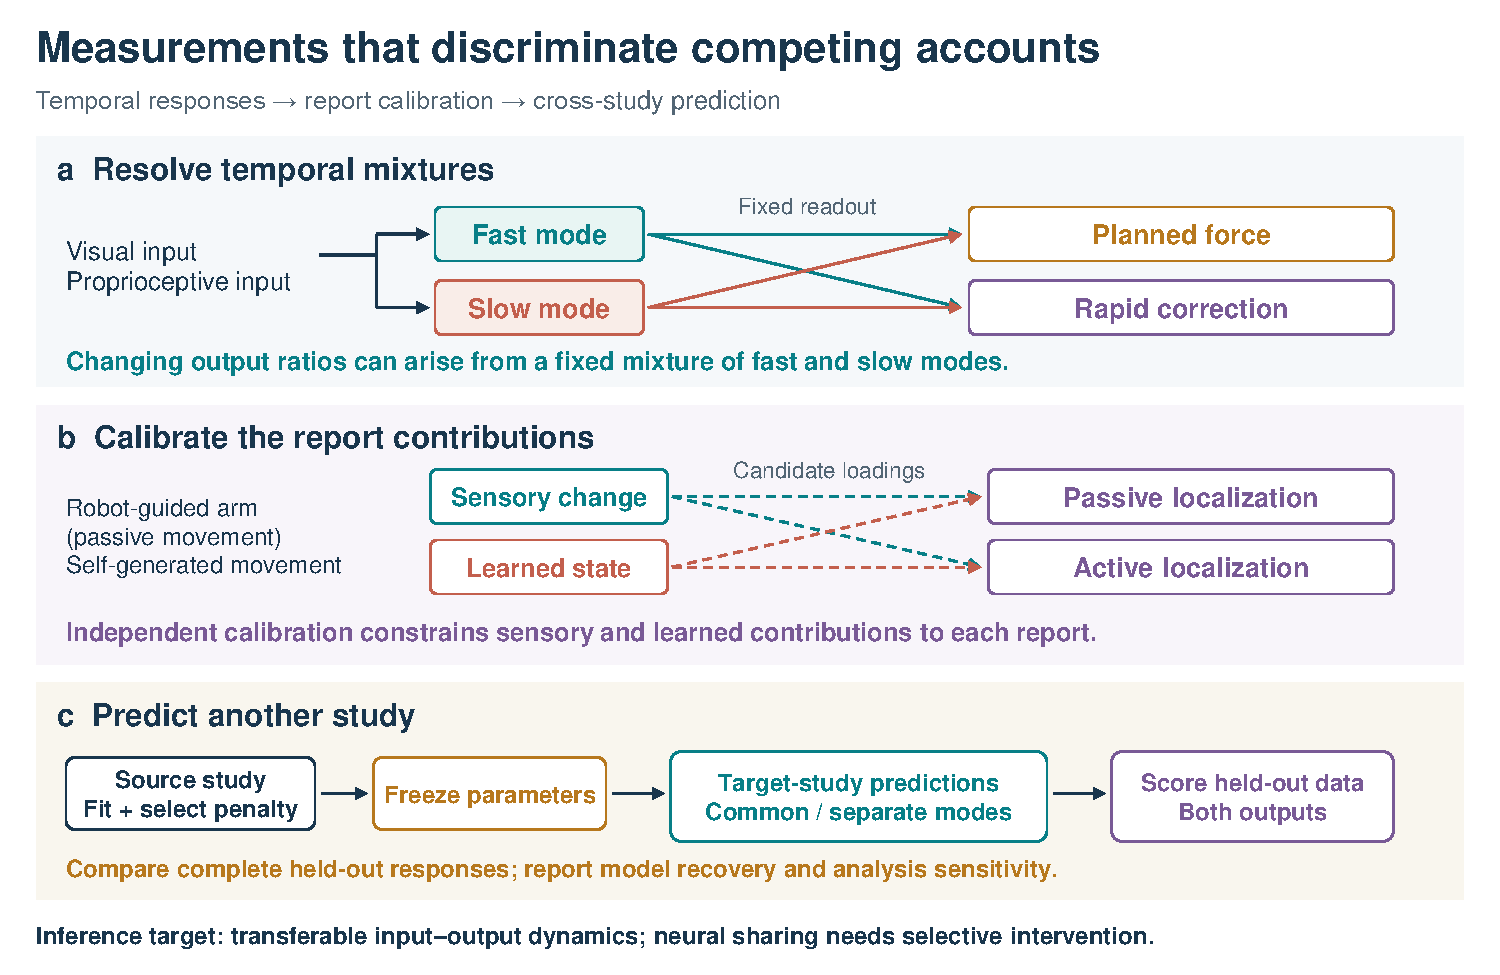
\includegraphics[width=\textwidth]{figure2_en.pdf}
\caption{Testing temporal mixtures, report loadings and external prediction. Fixed mixed readout can change delay ratios. Solid arrows connect temporal modes to the two measured outputs; dashed arrows denote candidate contributions to localization reports. Independent calibration constrains the report loadings. Passive movement denotes robot-guided human-arm movement. Source-fitted parameters are frozen before target-study scoring. The diagram is composed of native PowerPoint objects.}
\end{figure}
\FloatBarrier
\small\begin{longtable}{p{.20\textwidth}p{.34\textwidth}p{.36\textwidth}}
\caption{Evidence-derived choices of additional measurements. Full controls and simulation boundaries appear in the atlas.}\label{tab:rules}\\\toprule
Dispute & Minimal addition & Outcome interpretation\\\midrule\endfirsthead\toprule
Dispute & Minimal addition & Outcome interpretation\\\midrule\endhead\bottomrule\endfoot
R1 Shared updating versus context-dependent expression & Cross training and test cues; read the first probe before new error. & Test-cue effects identify expression; training effects persisting under a common test cue motivate updating/retention comparisons.\\[9pt]
R2 Input changes versus updating with mixed report loadings & Add active/passive reports and independent loading calibration; test report predictions in a new context. & Separated predictions support factor contrasts; unknown or collinear loadings retain a continuum of decompositions.\\[9pt]
R3 Fixed temporal copying versus integrated teaching signal & Add two error-onset times and a late sign reversal; record full correction, holding and next-trial waveforms. & Timing displacement supports copying; preserved learning timing with tonic-amplitude prediction supports integration.\\[9pt]
R4 Neural gain versus impedance & Add background EMG and multidirectional small mechanical perturbations, resolved by latency. & A stiffness change explains a mechanical contribution; residual response structure at matched mechanics constrains neural control.\\[9pt]
R5 Different acquisition versus different retention or probe-induced learning & Use independent first probes at multiple delays; counterbalance visual feedback during channels. & An early difference supports acquisition/readout effects; a later divergence directs attention to retention and probe exposure.\\[9pt]
R6 Common temporal modes with mixed readout versus output-specific modes & Measure both outputs over multiple independent delays and reserve new delays or histories. & A changing ratio rejects an effectively one-mode trajectory; common recurrences test shared temporal dynamics.\\[9pt]
R7 Mechanistic sharing versus statistical stabilization & Match effective regularization, optimize all competitors and evaluate recovery across realistic and near-equivalent instances. & Prediction advantage establishes predictive utility; mechanism selection additionally requires distinguishable intervention predictions and reliable recovery.\\[9pt]
R8 Task-error interaction versus strategic addition and attentional modulation & Cross task error with fixed cursor error, target flicker and instruction; collect matched aim reports plus immediate no-feedback aftereffects. & A residual task-error slope after aim and attention controls supports interaction; instruction-sensitive improvement with stable implicit aftereffects supports strategic addition.\\[9pt]
\end{longtable}\normalsize
\section{Frozen predictions across public human studies}
Two public force-field studies provide a test of how much temporal structure transports between experiments: one retained visual error information during adaptation and the other removed it (12 participants each). Both measured channel compensation and visually evoked force during abrupt and gradual field schedules. We compared one or two temporal modes, either common to both outputs or fitted separately. All models used the same source observations; parameter fitting and penalty selection preceded scoring on the other study's post-exposure data. These are retrospective predictions across studies. Supplementary Methods SM3 reports observation windows, baseline calibration, fitting, uncertainty and recovery procedures. \cite{franklin2021,franklin2023}

The strongest transported feature was temporal complexity (Fig.~3a,b). Adding a second common mode reduced joint standardized prediction MSE by 0.850 (95\% interval 0.472--1.296) from visual-error to visual-clamp training and by 0.459 (0.292--0.627) in the reverse direction. The gain was concentrated in anticipatory compensation. Feedback-force RMSE remained approximately 1.8--2.0 N, with a source phase template performing competitively. The result directs attention to the output carrying the predictive information: an improved joint score can be driven by the compensation trajectory.

Architecture ranking depended on how feedback was observed and models were regularized (Fig.~3c). In the primary window, separate-two minus common-two MSE was $-0.040$ (95\% interval $[-0.075,-0.002]$) in one transport direction and $-0.009$ ($[-0.027,0.008]$) in the reverse. The first direction changed sign in the secondary window, and unpenalized contrasts included zero. Thus the stable empirical finding is a richer compensation response; selecting a shared or output-specific organization requires predictions that remain separated across measurement choices. Complete endpoint scores and all comparisons remain in the Supplementary Evidence Atlas.

Fresh-instance recovery further localizes the available information. Under human residual noise, fitting abrupt exposure and predicting gradual exposure recovered 41 of 80 generating labels (51.2\%; four balanced families). Recovery was 7/20 and 4/20 for the one-mode common and separate families, respectively, and 15/20 for each two-mode family. This pattern supports a protocol-specific distinction in response complexity while showing uneven architecture discrimination. In addition, exact duplicated states can reproduce a common-state response. Together, prediction and recovery motivate the same experimental priority: measure joint responses under interventions that make the surviving explanations diverge.


\begin{figure}[!htbp]\centering
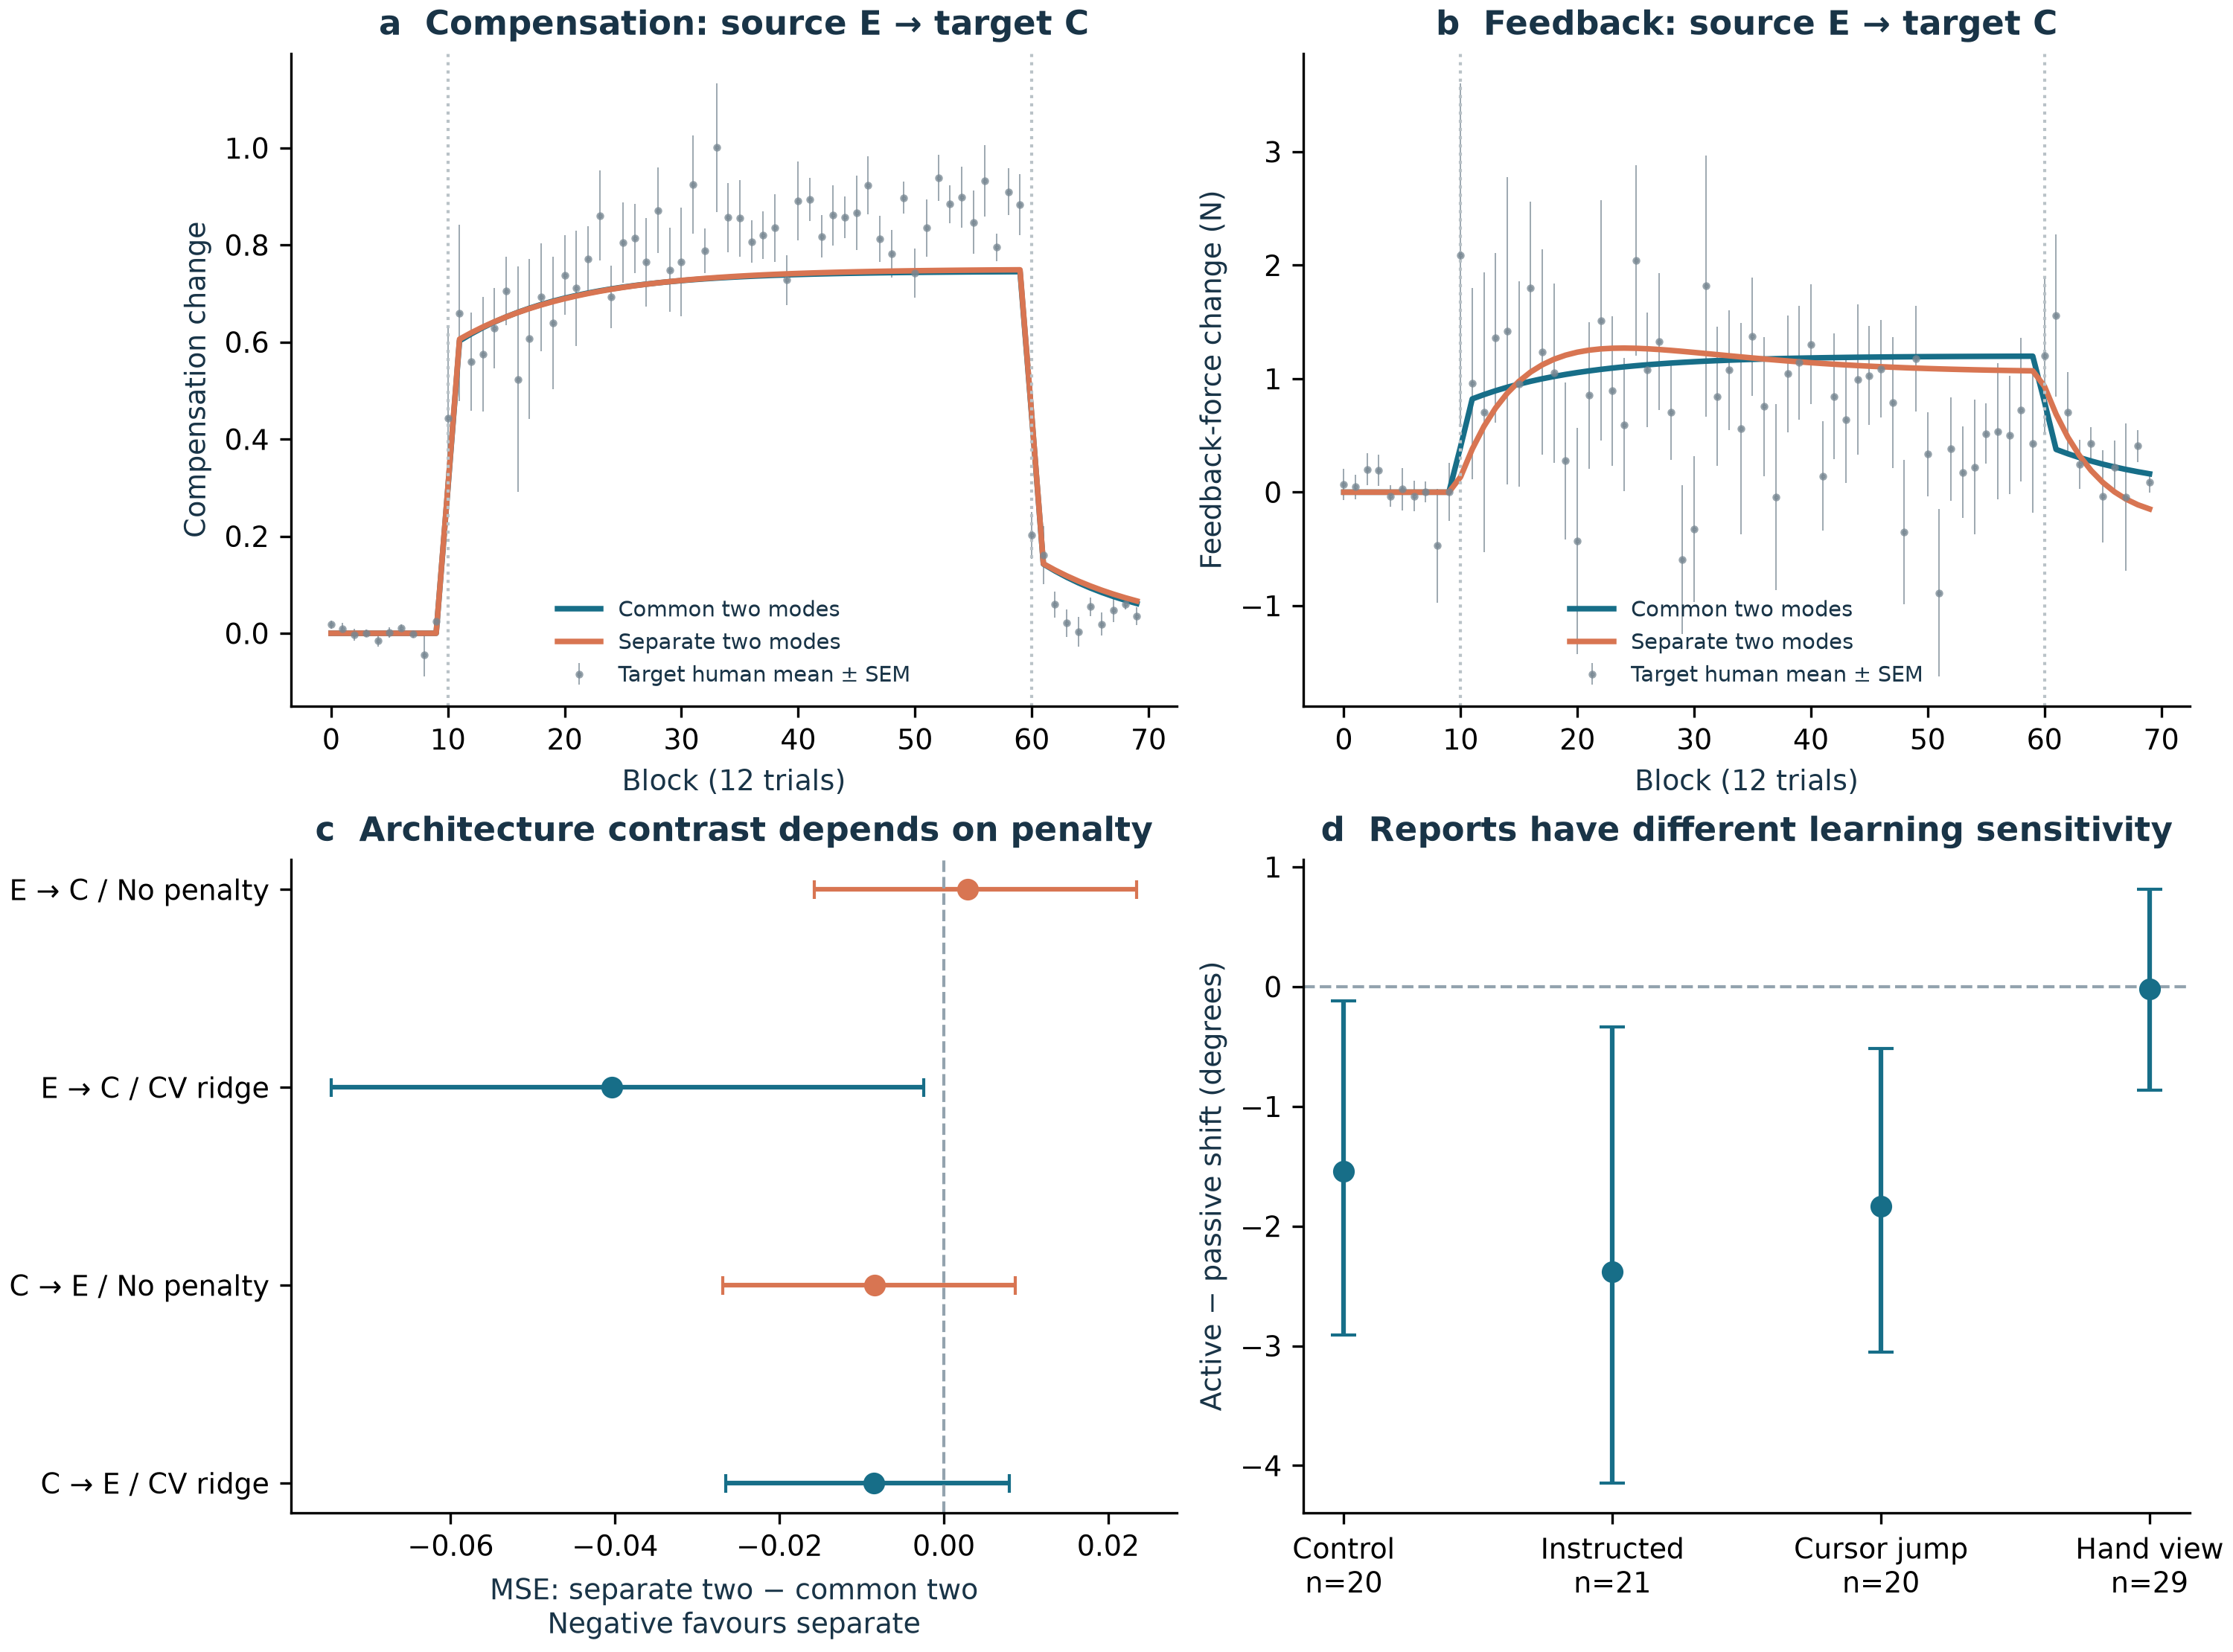
\includegraphics[width=\textwidth]{empirical_validation.png}
\caption{Public-data predictions and calibration checks. a,b: target-study mean changes (points, participant SEM) and frozen source predictions, shown for abrupt exposure; complete schedule scores are supplied. c: paired difference in joint standardized MSE, separate-two minus common-two, with target-participant bootstrap 95\% intervals. d: active-minus-passive localization shifts with participant-bootstrap 95\% intervals. Curves and points are computed from deposited human data; no image generation was used.}
\end{figure}
\section{What would move the explanation forward}
The synthesis yields a focused research agenda: locate the coupling that allows sensory-specific learning to influence planned and corrective actions. Three comparisons carry this agenda. Crossed training and test contexts identify when transfer depends on memory expression. Paired responses across delays test whether a changing transfer pattern follows common temporal components. Independently calibrated perceptual reports test whether sensory changes account for altered learning. Each comparison connects a particular uncertainty in the literature to a predicted consequence and a necessary measurement.

The strongest next biological test would combine distinct visual and proprioceptive errors with both anticipatory and corrective readouts, sampled under a common test context at reserved delays. Distinct input learning profiles together with cross-output transfer would support sensory-specific acquisition with convergent control consequences. Predicting those joint responses with fixed mixed readout would explain a delay-dependent dissociation within that architecture. Systematic held-out deviations would identify the input, context or temporal condition requiring a different account. Independent report calibration, mechanics measurements and matched probe exposure constrain the corresponding alternatives (Table~\ref{tab:rules}).

Embodied systems offer a prospective test of the measurement procedure. A microassembly controller can undergo separately documented changes in camera calibration, contact mechanics or memory, while placement accuracy is matched across implementations. Paired vision, contact-force and release measurements can then be tested for recovery of the changed component on a held-out part or surface. This experiment would establish whether the diagnostic transfers to a system with known interventions; comparable human measurements are needed to evaluate biological transfer.

Sharing becomes scientifically informative when its input, output, context and timescale are specified. Separability at acquisition and convergence at control can organize the same learning system. The evidence map and worked comparisons turn that integration into a practical question for each experiment: which additional observation would change the explanation of the joint response?

\section{Transparency and reproducibility}
The paired evidence records, frozen predictions, participant scores, model fits, exact counterexamples and executable scripts accompany this Perspective. Public data are secondary analyses of the cited studies. Target post-exposure observations were excluded from fitting and penalty selection. The analysis was developed after inspection of the broader archives and is retrospective. The accompanying recovery test uses newly drawn synthetic instances. Figures 1--2 were reconstructed in Microsoft PowerPoint as editable text and vector shapes with AI-assisted layout code; earlier drafts used OpenAI-generated conceptual images. The current figures contain no generated-image pixels. The quantitative figure is generated directly from analysis outputs. Language-model assistance supported literature organization, bilingual drafting and code preparation.
\section{Data availability}
This secondary analysis uses public human data from Franklin and Franklin (2021, 2023) and Gastrock et al. (2020). Source records and dataset identifiers are provided in the accompanying public\_data metadata. Processed block observations, participant localization estimates, model predictions and analysis summaries are included in the accompanying reproducibility package. \cite{franklin2021,franklin2023,external2020}
\section{Code availability}
The code and reproducibility package are available in the \href{https://github.com/WUJIAHAO-HKU/Shared-and-separable-motor-learning-reconciling-transfer-dissociation-and-error-attribution}{project repository}. The package contains the Python scripts for data extraction checks, temporal-model fitting, cross-study prediction, model recovery, calibration examples and quantitative figures. The README describes the workflow and dependencies; the release manifest records file hashes.
\section{Author contributions}
J.W. conceived the Perspective, organized the literature, performed the analyses, developed the code and wrote the manuscript. L.Z. provided supervision.
\section{Competing interests}
The authors declare no competing interests.
\section{Funding}
No specific funding was received for this work.

\begingroup\fontsize{8.5}{9.6}\selectfont\setlength{\parskip}{0pt}\setlength{\bibsep}{0pt}\bibliographystyle{unsrtnat}\bibliography{references}\endgroup\end{document}